\section{\benchname\space Framework}
% \pfliu{before diving into our RAGChecker, We need a subsection or even section to introduce some basics or preliminaries about (a) RAG setting, for example, what are retrieved contexts, generator, ground-truth answer. (b) existing typical evaluation methods for RAG }

\paragraph{Formulation} Define a modular RAG system as $\text{RAG} = \{\text{R}, \text{G}\}$, where $\text{R}$ is the retriever and $\text{G}$ is the generator. Given a query $q$ and documents $D$, it first retrieves top-$k$ relevant context $\{\text{chunk}_j\}=\text{R}(q, D, k)$, and then generates a model response $\text{m} = \text{G}(\{\text{chunk}_j\}, q)$. For simplicity, we can also represent the overall RAG generation process as $\text{m} = \text{RAG}(q, D)$. 

\paragraph{Design Principle} Given the compositional nature of RAG, we observe there are two major personae using a RAG evaluation framework. The first persona is a user that cares about the overall performance of RAGs and might choose a system with the best performance. Such a persona prefers a single value metric to compare and rank among RAG systems against a benchmark. The second persona is a developer that focuses on improving a RAG system with the need to identify causes of mistakes and potential rooms for improvements. Causes of errors in response can be classified into 1) retrieval errors, where the retriever fails to return complete and relevant context, and 2) generator errors, where the generator struggles to identify and leverage relevant information from context.

%1) completeness or relevance of retrieved chunks, 2) completeness or relevance in the generator’s self-knowledge, and 3) the generator’s capability in understanding and utilizing retrieved context and its self-knowledge. 

Consequently, metrics that reveal error causes should be different from those for overall performance, in the sense that error causes are module-specific or even reflected only by a certain behavior of a module. To help both personae to assess RAG performance, we design \benchname\space, a evaluation framework of RAG systems that consists of a benchmark with rich annotations and a set of diversely-purposed fine-grained metrics.

\subsection{Inputs to \benchname}

We prepare each sample in our benchmark dataset in the format of a tuple $\left< q, D, gt\right>$ representing query, documents, and ground-truth answer, where query is the input question to a RAG system, documents form the database providing possible context and are processed into chunks with the same number of tokens, and ground-truth answer is a complete and correct answer for the input question. Further information is provided in Sec.~\ref{sec:baseline_rag_systems}.

\subsection{Fine-grained Evaluation with Claim Entailment}

As illustrated in Fig.~\ref{fig:metrics}, a response generated by a RAG system might be a mixture of correct (\hollowcircle) and incorrect claims (\crossmark), while also missing some in-ground-truth claims (\hollowtriangle). In this sense, evaluating responses at a finer granularity is crucial to comprehensively assess the quality of an answer. For this purpose, we introduce two components: 1) a text-to-claim extractor that decomposes a given text $T$ into a set of claims $\{c_i\}$, and 2) a claim-entailment checker to determine whether a given claim $c$ is entailed ($\in$) in a reference text $Ref$ or not ($\notin$).% We implement claim extraction and entailment with RefChecker~\cite{hu2024refchecker}.\tong{need to remove the last sentence if refchecker is not mentioned before.}

%A response generated by a RAG system might contain a mixture of correct and incorrect statements, while missing some in-ground-truth claims. In this sense, evaluating responses at a finer grain is crucial to comprehensively assess the quality of an answer. For this purpose, we introduce two functions: 1) a text-to-claim extractor $\{C_i\} =f_\text{ext}(T)$, where $T$ is the text and $\{C_i\}$ represents the extracted set of claims, and 2) a claim-entailment checker  where $E_i = f_\text{chk}(C_i, \text{Ref})\in\{0, 1\}$ is a binary indicator of whether a claim $C_i$ is entailed in a reference text Ref. For simplicity, we also note $\{E_i\} = f_\text{chk}(\{C_i\}, \text{Ref})$ as a operation over each element in $\{C_i\}$.

\subsection{\benchname\space Metrics}
\label{sec:ragchecker_metrics}
With the annotation and claim-level entailment functions specified, we next define the metrics. For a RAG user, we design metrics to compare the performance among RAG systems, including a single-value F1 score as an overall metric. For a RAG developer, on the other hand, we propose two sets of modular metrics for the retriever and the generator in a RAG system respectively, that aim to decompose the system and diagnose the source of errors. In the rest of this section, we will first introduce the overall metrics and then go over modular metrics for retriever and generator separately. The formulas for each metric are summarized in Appendix~\ref{sec:appendix_formulation}.
%The design philosophy of all metrics is to produce claim entailment indicators with $f_\text{chk}(f_\text{ext}(T), \text{Ref})$ given any to-evaluate text T and reference text Ref, where each text can be model response, ground-truth answer, or retrieved chunks.




\begin{figure}[ht]
    \centering
    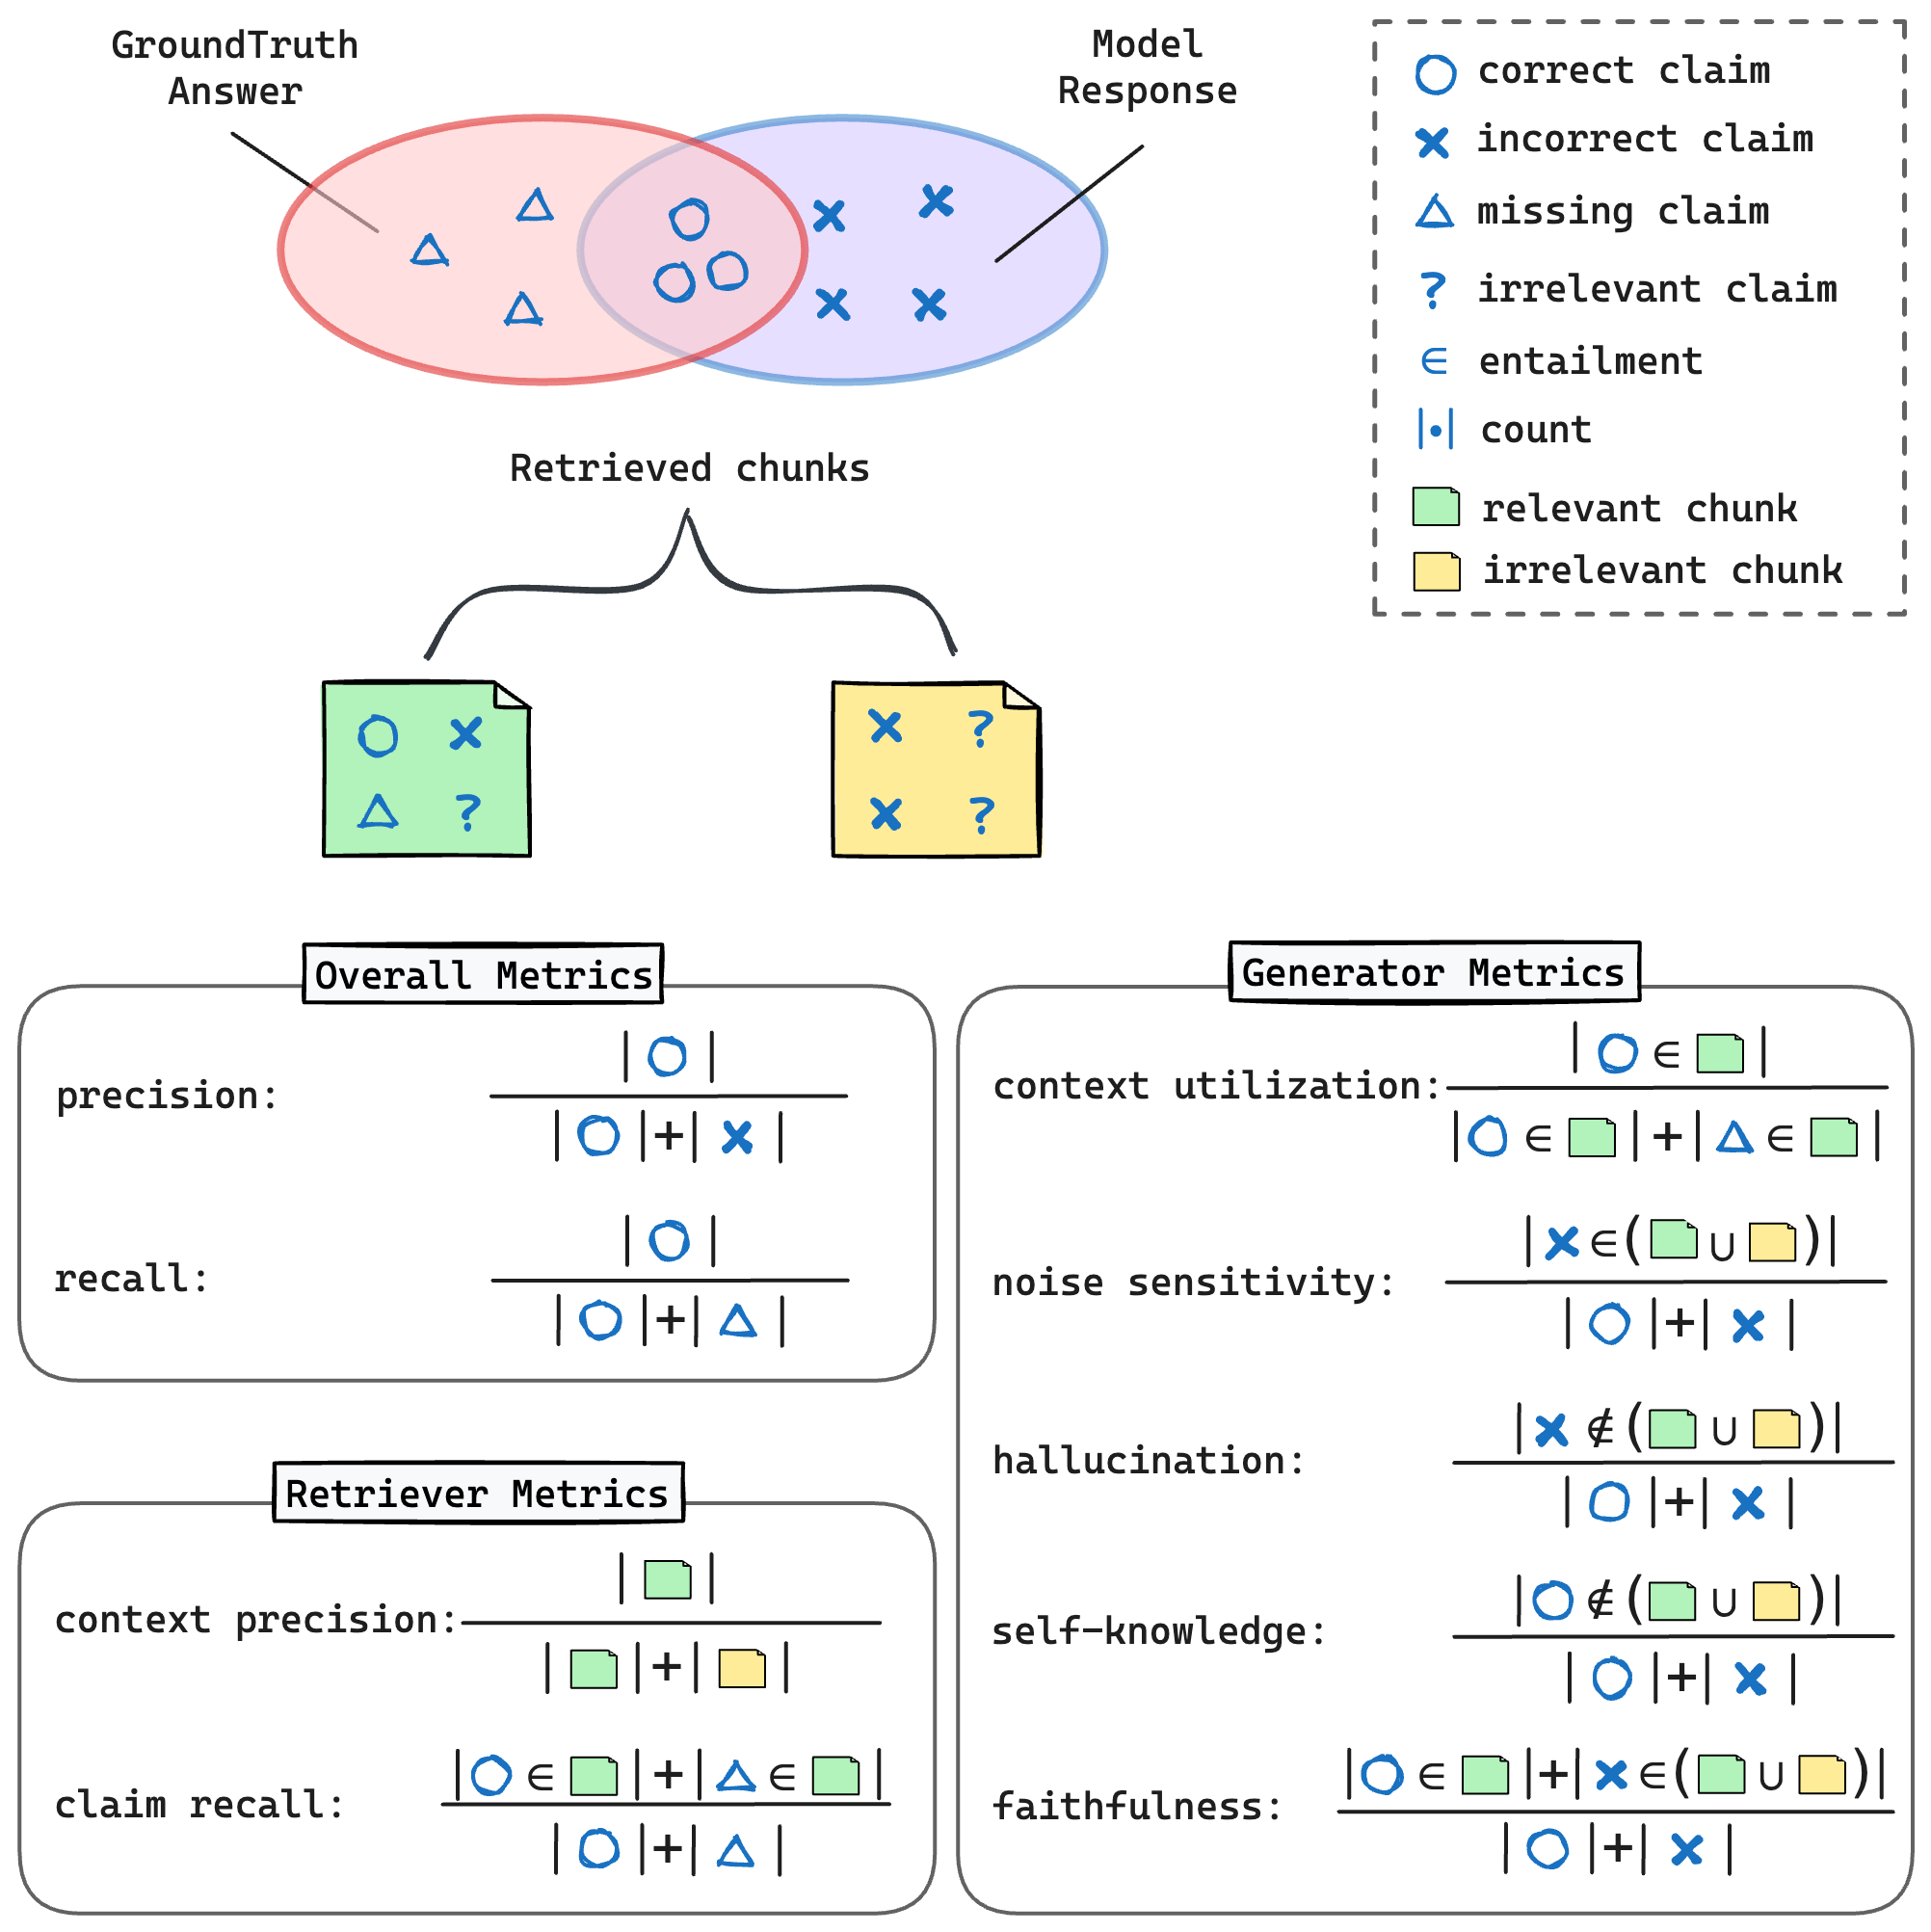
\includegraphics[width=0.7\linewidth]{figures/ragchecker_metric_simplified.png}
    \caption[]{Illustration of the proposed metrics in \benchname\space. The upper Venn diagram depicts the comparison between a model response and the ground truth answer, showing possible correct(\protect{\hollowcircle}), incorrect(\protect{\crossmark}), and missing claims(\protect{\hollowtriangle}). The retrieved chunks are classified into two categories based on the type of claims they contain. Below, we define the overall, retriever, and generator metrics, illustrating how each component of the RAG system is evaluated for its performance.}
    \label{fig:metrics}
\end{figure}

\subsubsection{Overall Metrics}

To assess the overall response quality of a RAG system from a user’s perspective, we can compute the precision and recall at claim level for each model generated response against its paired ground-truth answer. Specifically, we first extract claims from a model response $m$ and a ground-truth answer $gt$ as $\{c^{(m)}_i\}$ and $\{c^{(gt)}_i\}$ respectively. Then, we define correct claims in the response as $\{c^{(m)}_i|c^{(m)}_i\in gt\}$, and correct claims in the ground-truth answer as $\{c^{(gt)}_i|c^{(gt)}_i\in m\}$. Two metrics can be computed directly: \textbf{precision} is the proportion of correct claims in all response claims, and \textbf{recall} is the proportion of correct claims in all ground-truth answer claims. Further, the harmonic average of precision and recall gives the \textbf{F1} score, as the overall performance metric.

%compute $\{E^{(m)}_i\} = f_\text{chk}(\{C^{(m)}_i\}, \text{GT-A})$ and $\{E^{(gt)}_i\} = f_\text{chk}(\{C^{(gt)}_i\}, \text{Res})$ respectively. With $\{E^{(m)}_i\}$ we compute the response precision as $\sum_i \mathbb{I}(E^{(m)}_i = 1)/|\{E^{(m)}_i\}|$, i.e. the ratio of answer-entailed claims over all claims in the response. Similarly, we compute the response recall as $\sum_i \mathbb{I}(E^{(gt)}_i = 1)/|\{E^{(gt)}_i\}|$, i.e. the ratio of response-entailed claims over all claims in the answer. Further, the harmonic average of precision and recall gives the F1 score, as the overall performance metric.

%To assess the overall response quality of a RAG system from a user’s perspective, we can compute the precision and recall at claim level for each model generated response against its paired ground-truth answer. Specifically, we first extract claims from a model response $m$ and a ground-truth answer as $\{c^{(m)}_i\}$ and $\{c^{(gt)}_i\}=f_\text{ext}(\text{GT-A})$, and then compute $\{E^{(m)}_i\} = f_\text{chk}(\{C^{(m)}_i\}, \text{GT-A})$ and $\{E^{(gt)}_i\} = f_\text{chk}(\{C^{(gt)}_i\}, \text{Res})$ respectively. With $\{E^{(m)}_i\}$ we compute the response precision as $\sum_i \mathbb{I}(E^{(m)}_i = 1)/|\{E^{(m)}_i\}|$, i.e. the ratio of answer-entailed claims over all claims in the response. Similarly, we compute the response recall as $\sum_i \mathbb{I}(E^{(gt)}_i = 1)/|\{E^{(gt)}_i\}|$, i.e. the ratio of response-entailed claims over all claims in the answer. Further, the harmonic average of precision and recall gives the F1 score, as the overall performance metric.

\subsubsection{Retriever Metrics}

Ideally, a perfect retriever returns precisely all claims needed to generate the ground-truth answer. Completeness-wise, we can measure how many claims made in the ground-truth answer are covered by retrieved chunks. With retrieved chunks as the reference text, we compute \textbf{claim recall} as the proportion of $\{c^{(gt)}_i | c^{(gt)}_i \in \{\text{chunk}_j\}\}$.
%$\{E^{(gt)}_i\}=f_\text{chk}(\{C^{(gt)}_i\}, \{\text{chunk}_j\})$, and obtain the retriever recall as $\sum_i \mathbb{I}(E^{(gt)}_i = 1)/|\{E^{(gt)}_i\}|$.

Differently, we define the retriever precision at chunk-level instead of claim-level. A retrieved chunk is called \textit{relevant chunk} ($\text{r-chunk}$), if any ground-truth claim is entailed in it. In other words, $\text{chunk}_j$ is a relevant chunk if $\exists i, ~s.t.~ c^{(gt)}_i\in \text{chunk}_j$. The rest retrieved chunks are called \textit{irrelevant chunk} ($\text{irr-chunk}$). The retriever's \textbf{context precision} is defined as $|\{\text{r-chunk}_j\}|/k$, where $k$ is the number of all retrieved chunks.

Note that a chunk-level precision provides better interpretability than a claim-level one, because in practice RAG systems usually work with documents processed to be text chunks in a fixed size. That being said, it is likely that a chunk may contain relevant claims and irrelevant or misleading information at the same time. As a result, the best possible retriever can only achieve a claim-level precision score lower than 100\%, and such an upper-bound varies depending on the actual text distribution in $D$ and chunking strategy.

\subsubsection{Generator Metrics}

Given $k$ retrieved chunks (possibly mixing relevant and irrelevant information), a perfect generator would identify and include all ground-truth-relevant claims and ignore any that are not. Because the generator’s results have dependency on retrieved chunks, we provide in total six metrics characterizing different aspects of its performance.

Given a model response $m$ and its claims $\{c^{(m)}_i\}$, we first compute the proportion of $c^{(m)}_i$ that are entailed in retrieved chunks. This metric is \textbf{faithfulness}, as it describes how faithful the generator is to the provided context, thus the higher the better.

Next, we examine three types of incorrect response claims, i.e. $\{c^{(m)}_i | c^{(m)}_i \notin gt\}$.

\begin{enumerate*}

\item The first type includes incorrect claim that are entailed in a relevant chunk, then it indicates the generator is sensitive to noise coupled with useful information. The proportion of this type of claims to all $\{c^{(m)}_i\}$ is \textbf{relevant noise sensitivity}.
\item The second type includes incorrect claim that are entailed in an irrelevant chunk, then it indicates the generator is also sensitive to noise even in an irrelevant context. The proportion of these incorrect claims is \textbf{irrelevant noise sensitivity}.
\item Finally, the third type includes incorrect claims that are not entailed in any retrieved chunk, meaning all such claims are generated by the generator itself. Its proportion is \textbf{hallucination}.
\end{enumerate*}

Note that for simplicity we group the two noise sensitivities in Fig.~\ref{fig:metrics}, but later in Sec.~\ref{sec:analysis} we can see that generators generally has different sensitivity to relevant and irrelevant noise.

%Next, we compute $\{E^{(m)}_i\} = f_\text{chk}(\{C^{(m)}_i\}, \text{GT-A})$, and define those non-entailed claims, i.e. with $E^{(m)}_i = 0$, as incorrect claims. Incorrect claims can be further classified into three types.  By definition, other incorrect claims are entailed by a retrieved chunk. As discussed in Section 3.3.2, a chunk may come with a mixture of relevant and irrelevant information, and if an incorrect response claim is entailed to such a chunk, it means that the generator is sensitive to the noise in relevant chunks. This relevant noise sensitivity is computed as $|\{i |E^{(m)}_i = 0\& C^{(m)}_i\in\{\text{r-chunk}\}\}|/|\{E^{(m)}_i\}|$. Similarly, if an incorrect claim is entailed to a chunk with only irrelevant information, then it means the generator is sensitive to the noise in irrelevant chunks, therefore this irrelevant noise sensitivity is defined as $|\{i |E^{(m)}_i = 0\& C^{(m)}_i\in\{\text{irr-chunk}\}\}|/|\{E^{(m)}_i\}|$. All three metrics are expected to be low for a good generator.

Finally, we characterize how a generator uses information sources to produce correct claims. A correct claim not entailed by any chunk can only be based on generator’s \textbf{self-knowledge}, thus the proportion of these claims reflects how many correct claims are generated on its own. A lower self-knowledge score is better, when the generator is expected to fully depend on retrieved context only in a RAG system. On the other hand, we also check how much retrieved relevant information is used by the generator. Retrieved relevant information is measured by the number of ground-truth answer claims entailed in retrieved chunks, while the evidence of being used by generator is reflected by entailment in model response. Therefore, the \textbf{context utilization} is computed as the ratio between $|\{c^{(gt)}_i | c^{(gt)}_i \in \{\text{chunk}_j\}~\text{and}~c^{(gt)}_i \in m\}|$ and $|\{c^{(gt)}_i | c^{(gt)}_i \in \{\text{chunk}_j\}|$. Generally a higher context utilization is preferred.
